\documentclass[journal]{vgtc}                % final (journal style)
%\documentclass[review,journal]{vgtc}         % review (journal style)
%\documentclass[widereview]{vgtc}             % wide-spaced review
%\documentclass[preprint,journal]{vgtc}       % preprint (journal style)

%% Uncomment one of the lines above depending on where your paper is
%% in the conference process. ``review'' and ``widereview'' are for review
%% submission, ``preprint'' is for pre-publication, and the final version
%% doesn't use a specific qualifier.

%% These few lines make a distinction between latex and pdflatex calls and they
%% bring in essential packages for graphics and font handling.
%% Note that due to the \DeclareGraphicsExtensions{} call it is no longer necessary
%% to provide the the path and extension of a graphics file:
%% 
\includegraphics{diamondrule} is completely sufficient.
%%
\ifpdf%                                % if we use pdflatex
  \pdfoutput=1\relax                   % create PDFs from pdfLaTeX
  \pdfcompresslevel=9                  % PDF Compression
  \pdfoptionpdfminorversion=7          % create PDF 1.7
  \ExecuteOptions{pdftex}
  \usepackage{graphicx}                % allow us to embed graphics files
  \DeclareGraphicsExtensions{.pdf,.png,.jpg,.jpeg} % for pdflatex we expect .pdf, .png, or .jpg files
\else%                                 % else we use pure latex
  \ExecuteOptions{dvips}
  \usepackage{minted}
  \usepackage{graphicx}                % allow us to embed graphics files
  \DeclareGraphicsExtensions{.eps}     % for pure latex we expect eps files
\fi%

%% it is recomended to use ``\autoref{sec:bla}'' instead of ``Fig.~\ref{sec:bla}''
\graphicspath{{figures/}{pictures/}{images/}{./}} % where to search for the images

\usepackage{microtype}                 % use micro-typography (slightly more compact, better to read)
\PassOptionsToPackage{warn}{textcomp}  % to address font issues with \textrightarrow
\usepackage{textcomp}                  % use better special symbols
\usepackage{mathptmx}                  % use matching math font
\usepackage{times}                     % we use Times as the main font
\renewcommand*\ttdefault{txtt}         % a nicer typewriter font
\usepackage{cite}
\usepackage{caption}
\usepackage{array}

%% If you are submitting a paper to a conference for review with a double
%% blind reviewing process, please replace the value ``0'' below with your
%% OnlineID. Otherwise, you may safely leave it at ``0''.
\onlineid{0}

%% declare the category of your paper, only shown in review mode
\vgtccategory{Research}

%% Paper title.
\title{Visualizing the Los Angeles Metro Bikeshare System}

%% This is how authors are specified in the journal style
%% indicate IEEE Member or Student Member in form indicated below
\author{Prathyusha Butti, Pratik Bhandari and Ripan Chowdhury}
\authorfooter{
%% insert punctuation at end of each item
\item
 \author{Prathyusha Butti, Pratik Bhandari and Ripan Chowdhury}
 are graduate students at the University of Arizona.
 
E-mail:pbutti@email.arizona.edu. 
E-mail:pratikbhandari@email.arizona.edu.
E-mail:rchowdhury1@email.arizona.edu.
}

%other entries to be set up for journal
%\shortauthortitle{Firstauthor \MakeLowercase{\textit{et al.}}: Paper Title}

%% Abstract section.
\abstract{
Bike sharing systems are gaining immense popularity as an alternative or complementary mode of urban transport. Bike sharing can provide an alternative to traditional modes of transport or, more likely a complementary service for solving the "last mile problem" of getting from a public transportation stop to the final destination. Furthermore, bike sharing systems may help mitigate automobile congestion and reduce pollution, although relatively little research has been done to asses their actual impact in these areas. Visualizing and analyzing the current operations can assist in getting a better grasp on the performance of the system. In this paper, a data visualization approach is used to identify important factors related to the bike-sharing system. We analyze the bike-sharing system such that we are able to group the bike renting trends, locate the busiest stations in the locality and number of monthly or flex passes taken by the customers for different time granularity. We mine the Metro Bike Share, Los Angeles data and discuss the findings of this data set. Using this publicly available data, we conduct some experiments combining data filters and visualizations, potentially analyzing the sustainability of the bike sharing system.
For this milestone, we have expanded on our progress from the second milestone. One of the major tasks was to work on the development of the map visualization. Along with learning the tools and techniques required for developing the visualization, we worked on the initial data acquisition and cleanup process as well. Besides that, we have worked on the refinements that were suggested from the second milestone.

} % end of abstract

%% Keywords that describe your work. Will show as 'Index Terms' in journal
%% please capitalize first letter and insert punctuation after last keyword
\keywords{Bike-Share, Visualization, Clustering, Data Mining.}

%% ACM Computing Classification System (CCS). 
%% See <http://www.acm.org/class/1998/> for details.
%% The ``\CCScat'' command takes four arguments.

%\CCScatlist{ % not used in journal version
% \CCScat{K.6.1}{Management of Computing and Information Systems}%
%{Project and People Management}{Life Cycle};
% \CCScat{K.7.m}{The Computing Profession}{Miscellaneous}{Ethics}
%}

%% Uncomment below to include a teaser figure.
%   \teaser{
%   \centering
%   \includegraphics[width=16cm]{CypressView}
%   \caption{In the Clouds: Vancouver from Cypress Mountain.}
%  }

%% Uncomment below to disable the manuscript note
\renewcommand{\manuscriptnotetxt}{}

%% Copyright space is enabled by default as required by guidelines.
%% It is disabled by the 'review' option or via the following command:
% \nocopyrightspace

\vgtcinsertpkg

%%%%%%%%%%%%%%%%%%%%%%%%%%%%%%%%%%%%%%%%%%%%%%%%%%%%%%%%%%%%%%%%
%%%%%%%%%%%%%%%%%%%%%% START OF THE PAPER %%%%%%%%%%%%%%%%%%%%%%
%%%%%%%%%%%%%%%%%%%%%%%%%%%%%%%%%%%%%%%%%%%%%%%%%%%%%%%%%%%%%%%%%

\begin{document}

%% The ``\maketitle'' command must be the first command after the
%% ``\begin{document}'' command. It prepares and prints the title block.

%% the only exception to this rule is the \firstsection command
\firstsection{Overview} % or "Motivation"

\maketitle

\label{sec:overview}
Bike share schemes are an increasingly prevalent mode of intra-city transportation. The concept of bike sharing systems was introduced in 1965 Amsterdam. A bike sharing program is a system of supplying bikes for hire for point-to-point transportation. This program enables convenient active transportation as people have an option to ride between two stations in a defined geographical area. Since the introduction of bike-sharing systems, much research has been dedicated to different aspects of these systems. The benefits of bikes in urban areas, where travel distance is short, and the parking prices are high, has caused the demand for bike-sharing systems to increase. Bike share systems may help mitigate automobile congestion and reduce pollution, although relatively little research has been done to assess their actual impact in these areas. Benefits to users include potentially reduced commute times by perhaps as much as 10\% \cite{Sakari:2013:Data} and a healthier lifestyle to lead. 
 
Besides visualizing bike sharing systems as a new means of public transportation, such community shared programs offer a new way to look into the dynamics of movements inside a city, and more generally into its activity. In a sense, it provides digital footprints that reveal the activity of people in the city over time and space and makes possible their analysis. Different issues motivate the study of such a system. Some questions are about the usage patterns of this kind of transport, with reference to social or economic studies of transportation, while others are about the system itself: does the service work correctly? Can it be optimized? Can one regulate the availability of bikes? Some of the studies related to this system are descriptive and mine the data to get a better understanding of the operations. 

Data Visualization and analysis of the current operations can assist in getting a better grasp on the performance of the system. Data visualization, which is defined as the effort of placing data in a visual context, can assist in better understanding the problem. When we have many data points, the visualization of the data becomes challenging. The purpose of this study is to analyze the bike-sharing system by applying filters like renting trends. We have mined the Metro Bike Share, Los Angeles data and discussed the findings of this data set. We have examined the bike-share system during different quarters of the year, therefore potentially analyzing the sustainability of the bike sharing system. This study also helped us in gaining a better understanding of the urban mobility of Los Angeles residents. In terms of visualizations, our project does not develop a novel visualization but uses prevalent methods of visualizing data to try and find trends of a certain behavior from this dataset. We have analyzed various types of visualizations and brought together several ideas to form an interactive and easy-to-use interface that helps users navigate through the bike-sharing data in a more ordered and systematic way. Our choice of visualization holds ground with the design practices that make an effective visualization and also takes into consideration some design techniques that further enhance the user experience.

The following progress has been made for this milestone:
\begin{itemize}
  \item \textbf{Presentation}: We have a presented our visualization on November 21st, 2018 to the class and recieved their feedback.  
  \item \textbf{Evaluation}: We have designed our evaluation and received results from different users and have analyzed them in the evaluation section.

\end{itemize}
 

\section{Technical Progress} 
\label{sec:technical_progress}

Continuing from the progress in the second milestone, we started implementation of the chosen visualization design. This involved a number of steps that were carried out over the course of two weeks that resulted in a visualization that now forms the basis of our future progress. The contributions made in service of this visualization design are explained in separate subsections below,

\subsection{Data Collection}
\label{sec:data collection}

The data used for the visualization was collected from the database of \textbf{Bike Share Metro}, a bike share service based in Los Angeles. This is a completely open source data that provides us with various information about any single bike ride. A more detailed description of all the fields in the data can be found in the Task Abstraction subsection of the Refinements section.\\
The data is divided into several segment, each one contained the information for a single quarter of a calendar year i.e. Q1, Q2, Q3 or Q4. After downloading the data from their online database, the resulting .zip archive was extracted. The raw data was provided in a CSV (Comma Separated Value) format.

\subsection{Data Refinement and Restructuring}
\label{sec:data refinement and restructuring}

The raw data in the CSV format is not suitable for processing and analysis. We used a more standard approach to work with data and for this the CSV data files were converted into JSON (JavaScript Object Notation) format. All of the data cleaning and pre-processing was done using the \textbf{Python} programming language. This reformatting of the raw data structure was followed by a series of further transformation which are explained in the sub-sections below.

\subsubsection{JSON Format}
As mentioned above, the first step was to convert the raw data from CSV to JSON format. Other than the structure of the data, the contents were left intact and no further manipulations were done to the data.\\
The script \texttt{csv\_to\_json.py} in the \textbf{Project} folder performs this initial conversion.

\subsubsection{GeoJSON Format}
While the JSON data format in itself is pretty suitable for data analysis and works very well for our purposes, GeoJSON is a format that works even better when visualizations involve geographic maps and latitude, longitude locations. During this process, we also performed data cleaning operations where data containing incomplete information were not loaded into the GeoJSON data structure.\\
The script \texttt{json\_to\_geojson.py} in the \textbf{Project} folder converts the JSON file into a GeoJSON data structure.

\subsubsection{Task-Specific Formats}
Following the GeoJSON re-formatting and data cleanup, the data structures for specific visualization mappings are created. The GeoJSON file is taken as the base file from which all other dictionaries and arrays of information are extracted.\\
For our current visualization progress, we have a single extraction from the GeoJSON file. This dictionary contains the distinct geographic locations of all bike pickup points along with the number of pickups for that time frame (1st quarter of 2018 in our case). This is done by the \texttt{geo\_to\_startcount.py} script in the \textbf{Project} directory.\newline\\ It should be noted that for every new visualization design or task, a new data structure will be extracted from the GeoJSON file to ease the data analysis and extraction process.
Currently, all these scripts exists in standalone and need to be executed one after the other. On the final implementation, these scripts will be a part of a single executable script which will perform all the data cleaning and manipulation tasks in a single execution.

\subsection{Data Visualization}
Following the data collection and restructuring, we proceeded towards the actual visualization of the data. The visualization process along with the different tools and packages used in support of that have been explained in the subsections below.

\subsubsection{Initial Map Layout}
The first task at hand was to lay out a map of Los Angeles over which we had to plot our data points. Though D3 in itself supports drawing maps, we required a detailed street level map layout. For this purpose, D3 could not be used alone. We had to use a separate package or library that supports interactive map drawing. We had two possible options to work with for our visualization, \textbf{Google Maps API} and \textbf{Leaflet}.\\
There did not seem to be a large difference between the functionalities provided by Google Maps and Leaflet, at least for our visualization purposes. While Google Maps did was a fan favorite among a large number of developers and it did provide many added features in terms of traffic, transit data and geolocation, we decided to implement Leaflet into our project. Our decision was based on the availability and simplicity of the documentation and tutorials for these features. Leaflet conformed to our requirements smoothly and its implementation was pretty straight forward.\\
In essence, Leaflet is a open-source JavaScript library for interactive maps \cite{Leaflet:2017:Doc}. It is light weight and consists of a plethora of features that can be implemented for interactive map visualizations. For our visualization, we create the map in the 'map' div and add \textit{OpenStreetMap} tiles to load the map area. As a starting point, we provide the map with a fixed co-ordinate and a zoom level. Using this information, an initial visual representation of the map is obtained. From here, users can further interact with the map. The interactions supported in our visualization are discussed in detail in a later section.
\begin{figure}[h]
	\centering % avoid the use of \begin{center}...\end{center} and use \centering instead (more compact)
	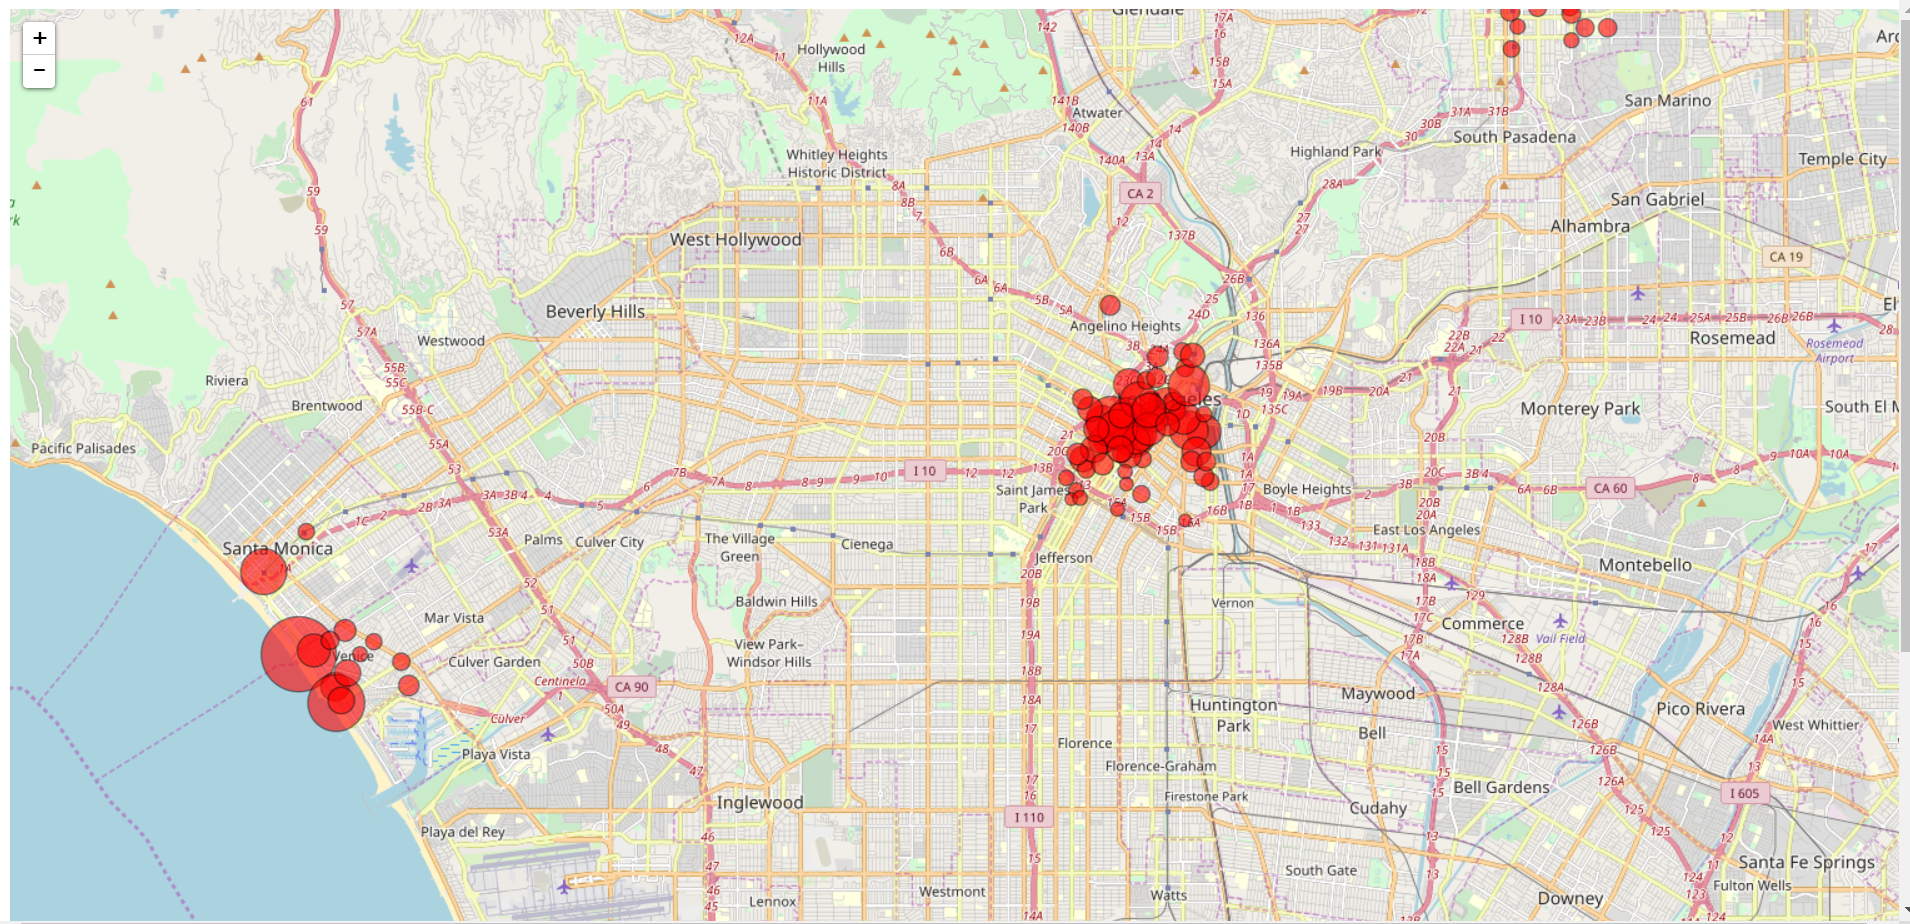
\includegraphics[scale=0.20]{figs/highlevel.PNG}
	\caption{\footnotesize{A high-level overview of current visualization}}
	\label{fig:First viz Chart}
	\captionsetup{justification=centering,margin=1cm}
	\vspace{-10pt}
\end{figure}
\subsubsection{Data Plotting}
After plotting the map of Los Angeles, we started with plotting the data points over this map. For the first visualization, we plotted the starting locations of all bike rides over the map. These were distinct locations in the map, defined by a latitude and longitude value. We used the data for the 1st quarter of 2018 as our seed data. The number of data points were in the order of 60,000 for a single quarter. For now, this data is loaded locally but as we include more data points for different quarters and years, we are planning to shift the data loading through a web server. This will considerably decrease the load time of the visualization.\\
The data points for our visualization are represented as circles of varying area (radius). The data is encoded in such a way that the radius linearly increases with the frequency of bike pick-ups for a given location. We keep the opacity of the circles to a value less than 1 so as to make the map visualization easier to understand and navigate. These circles are stroked with a minimum thickness to make them stand out when viewing from a zoomed-out perspective.
\begin{figure}[h]
	\centering % avoid the use of \begin{center}...\end{center} and use \centering instead (more compact)
	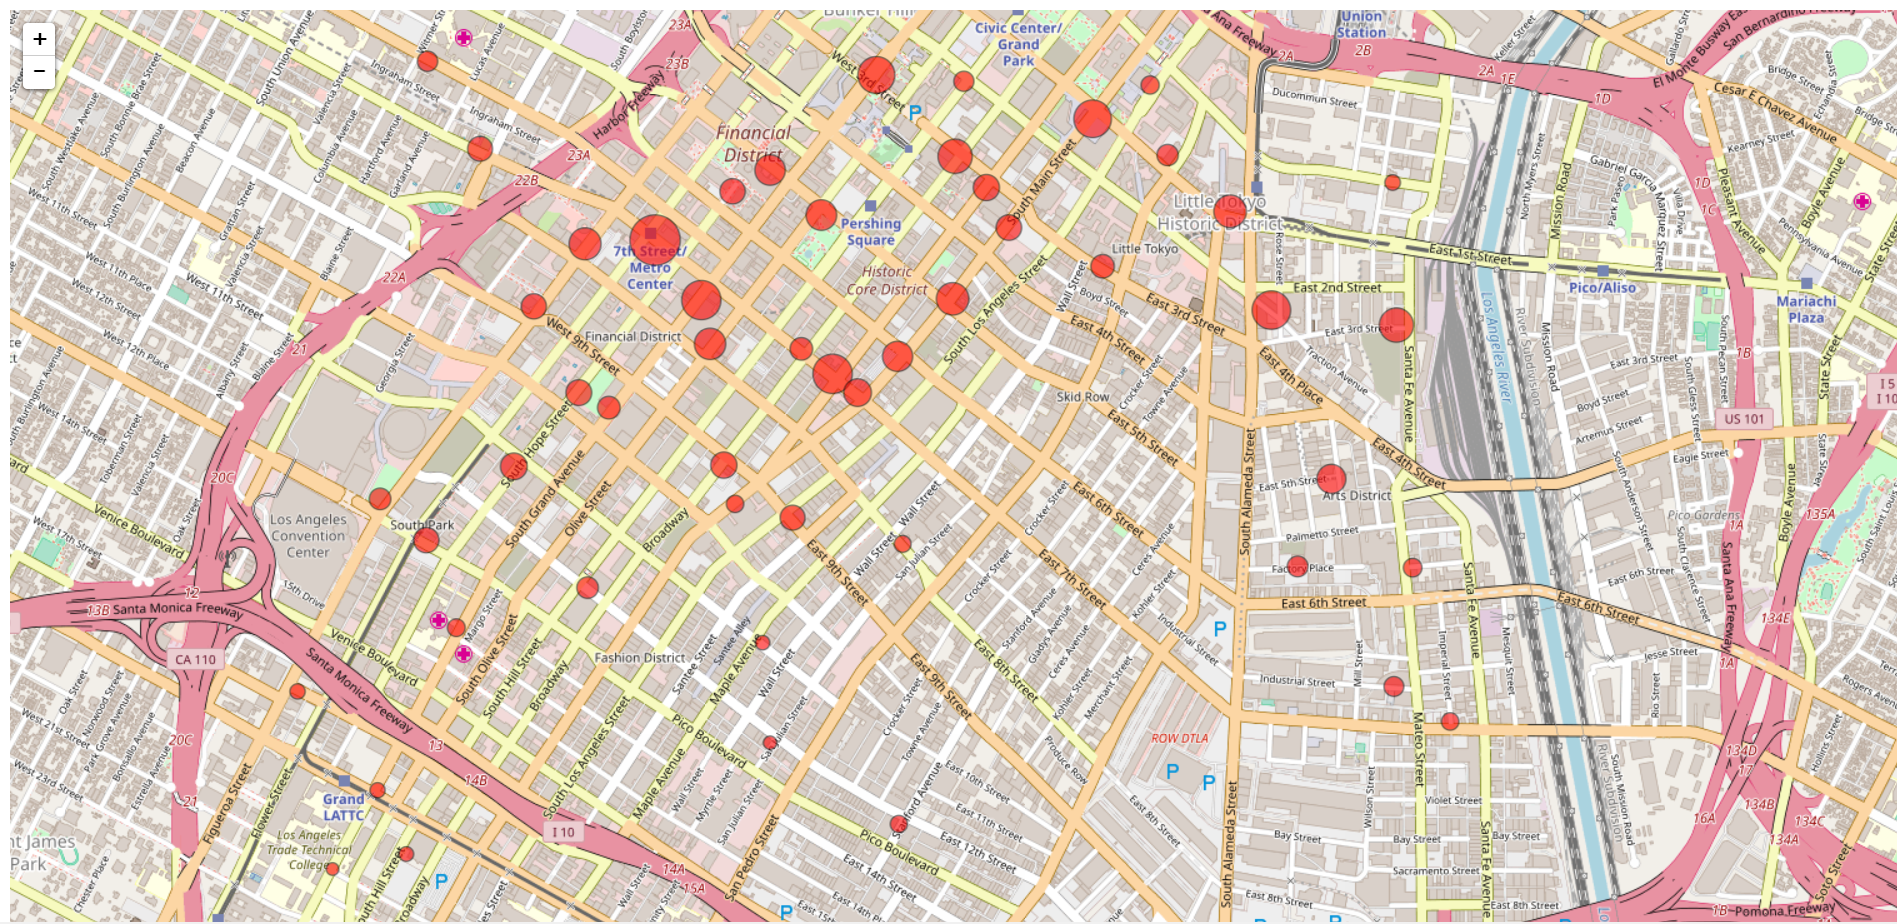
\includegraphics[scale=0.20]{figs/zoomedin.PNG}
	\caption{\footnotesize{A zoomed in view showing distinct geographic points}}
	\label{fig:First viz Chart}
	\captionsetup{justification=centering,margin=1cm}
	\vspace{-10pt}
\end{figure}
\subsection{User Interaction}
Our visualization design currently supports a number of interactions. These visualizations have been presented in the short movie as well. As work progresses on the visualization, these interactions will be enhanced and others added. For now, the following interactions are available to the user:
\begin{itemize}
    \item \textbf{Panning and Zooming}: The geographic map can be panned sideways to move around and locate different data points around the city. Also, the map can be zoomed in and out. Zooming in allows users to get a closer look into the data points on a street level view. This way the bike stations look more distinguishable from one another. The zoom feature here is constrained and semantic in nature. This interaction follows the Shneiderman's mantra of having an overview first and then allowing to zoom in and filter data.
    \item \textbf{Pop-up Effect}: The individual data points support a "On Click" feature. Every time a data point i.e. a circle is clicked, the color of the circle changes to blue with a more defined stroke around the circle. This makes the data point more visible and allows it to stand out, especially when there are a large number of similar data points around it. We decided on choosing the "On Click" action to show the effect rather than the "Hover" action since clicking an element to have a detailed overview of a single data point is more effective than hovering over it. Either ways, this follows the Shneiderman's Detail-on-Demand task taxonomy.
    \item \textbf{Tooltip}: In addition to the "On Click" feature changing the color of the circle, a tooltip will also appear on top of each data point. Currently, this tooltip shows the number of bike pick ups for a given location but a future enhancement might be to add a small visualization pertaining to the data within that geographic point.
\end{itemize}
\begin{figure}[h]
	\centering % avoid the use of \begin{center}...\end{center} and use \centering instead (more compact)
	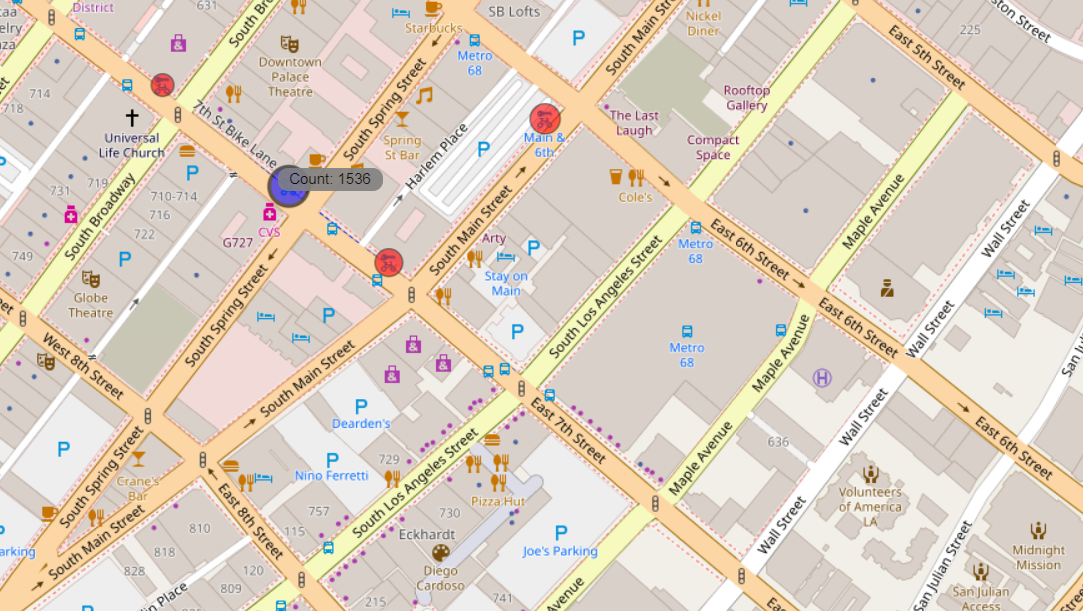
\includegraphics[scale=0.36]{figs/tooltip.png}
	\caption{\footnotesize{A simple tooltip implementation}}
	\label{fig:First viz Chart}
	\captionsetup{justification=centering,margin=1cm}
	\vspace{-10pt}
\end{figure}
This visualization has been coded by dividing the structure of the program into 3 segments:
\begin{itemize}
    \item PM3.html
    \item PM3.js
    \item PM3.css
\end{itemize}
As work progresses on the visualization, we plan on adding a histogram time frame at the bottom of the visualization window. This histogram will stretch the width of the window and allow users to cross-filter data in the map based on the selection in the histogram window.

%%\section{Task and Data Abstraction} 
\label{sec:task_and_data_abstraction}

We initially obtained our data from a popular online data source, Kaggle. The dataset was named \textit{Los Angeles Metro Bike Share Trip Data}. Even though this dataset had enough depth to reason about various trends and patterns, it was less in number which made us look for other sources of similar data. We then found a substantial amount of data in Bike Share Metro, which seemed to fulfill our requirements for this project. This data, like the one before, is from Los Angeles and contains the shared bike ride information for 2.5 years, 2016 Q3 to 2018 Q2. 
The dataset is in Table form and the table has all total 14 attributes. They are:
\begin{itemize}
    \item trip\_id - Unique ID for a particular trip
    \item duration - Duration of the trip in minutes
    \item start\_time - Start time of the trip
    \item end\_time - End time of the trip
    \item start\_lon - Starting position longitude
    \item start\_lat - Starting position latitude
    \item start\_station - The station ID where the trip originated
    \item end\_station -  The station ID where the trip terminated
    \item end\_lat - Destination latitude
    \item end\_lon - Destination longitude
    \item bike\_id - Id for each bike
    \item plan\_duration - Duration of the customer's plan
    \item passholder\_type - The name of the pass holder's plan
    \item trip\_route\_category\ -  "Round Trip" for trips starting and ending at the same station or "One Way" for all other trips
\end{itemize}
Moreover, there are four spatial attributes in the datasets, namely, start\_lon, start\_lat, end\_lon and end\_lat. We will be using the trip\_id as the key for each item.

\subsection{Task Abstraction}
\label{sec:task}
All the data about bike share venture we could gather focus mainly on the number of customers, duration of their trips and the locations from which the bikes are rented. So, our aim is to analyze which places see the maximum number of business each day, moreover how the business is growing over time. The goals identified by us are the following:

\begin{itemize}
    \item G1: Get a mental picture of business according to location:
    It will be very helpful in analyzing the viability of the bike share system if we could get a mental picture, around which geographic locations most of the business tend to gather. If there was a visible comparison between different locations, it would be so much easier to comprehend where the focus of the business should be, moreover if we can find some connection between high volume of the rentals at those locations, the same model could also be implemented in other locations with similar potential. The idea of business can be explained by the number of drop-offs and hires from a specific station. Typically, a station having a high number of hires has more business. We will also check for stations where both drop-offs and hires are high. These can be considered as locations with high business. By mapping the drop-off i.e. (end\_longitude, end\_latitude) and hire i.e. (start\_longitude, start\_latitude) over the geographic map, we can get a good sense of our task.

    \item G2:  How the customers’ preferences are changing over time
    There are three kinds of passes available for the customers, namely walkup (daily), monthly and flex (annual). They provide one day, one month and year-round rental service respectively. If we could find the trends in the change in the number of passes over different time granularity, we could get a clear picture of the preferences of the customers. The time granularity can be either months or quarters or years.
    
    \item G3: How the volume of the rentals changes over time:
    If we can visualize how the number of customers changes over time, it will also provide us with clarifications about which time of the year people tend to chose this form of transport over others. That would be beneficial to understand what compels them to eschew bikes over the other time of the years and what steps could be taken to alleviate their discomfort.
 
\end{itemize}

To identify the smaller task in support of the goals, we can take the following steps.

\begin{itemize}
    \item T1: Comparing the aggregate rentals from different regions:
    We can try to visualize the number of rentals from different geographic locations from the start\_lon and start\_lat attributes from the dataset. The total number of customers from the specific bike stations from different locations can be helpful in getting insights about the viability and the fruitfulness of this venture in different locations.

    \item T2: Comparing rentals at different time of the years:
    We have the data on the number of rentals according to the different quarters of the years from 2016 to 2018. So if the user wants to zoom into the visualization using a context + focus design approach, it would also be apparent how the number of rentals is changing along the different times of the year.

    \item T3: Comparing the passes throughout the years:
    We can make the comparisons between the different kinds of passes over different quarters/months of different years. We can show this way how many passes from the three categories are getting sold each at each time level. Moreover, it can give us some insights about which pass generates the most amount of revenue and which one is the best option for holding on to customer loyalty and thus garnering and maintaining the reputation for the company.
\end{itemize}

Summary: All the visualizations necessary here tend to focus on the comparisons, discovery, and identification to some extent. We can use these task abstractions and objectives as further guides to our design selection process.

%%\section{Preliminary Designs} 
\label{sec:preliminary_designs}

In the course of research and discussions about possible visualization to implement for our project, we came up with a number of suitable visualizations that seemed suitable to use in our project. Below is the list and description of each visualization along with reasoning to support our choice of this visualization.

\subsection{Pick-Up vs Drop-Off}
\label{sec:viz1}

The first design we thought of was a geographical map which plots the arrival and departure areas of the share-bikes and maps this data according to their frequency. So, for this visualization, a geometrical plot was being used. Here the marks were the share-bikes (either arriving or departing) and the attribute was the frequency of arrival or departure. We planned on using circles to denote the arrival or departure at the bike station. This way, the mark of the visualization could be considered as a circle. Since we will be mapping both the arriving and departing bikes, it would be confusing to have circles of both types of data of the same color. Hence, we decided to denote departing and arriving bikes by red and blue color respectively. Similarly, the frequency of arrival/departure would be encoded by the area of the circle (encoding rule). The channels here are the geographical (x and y) positions, color and area. 

This choice of visualization was directly influenced by similar work \cite{UrbanDataCyclist} done by Daniel Peterson, where they mapped hires and drop-offs on a location with circles and encoded the frequency with the area of the circle. The following design is from the above-mentioned study itself.
\begin{figure}[h]
	\centering % avoid the use of \begin{center}...\end{center} and use \centering instead (more compact)
	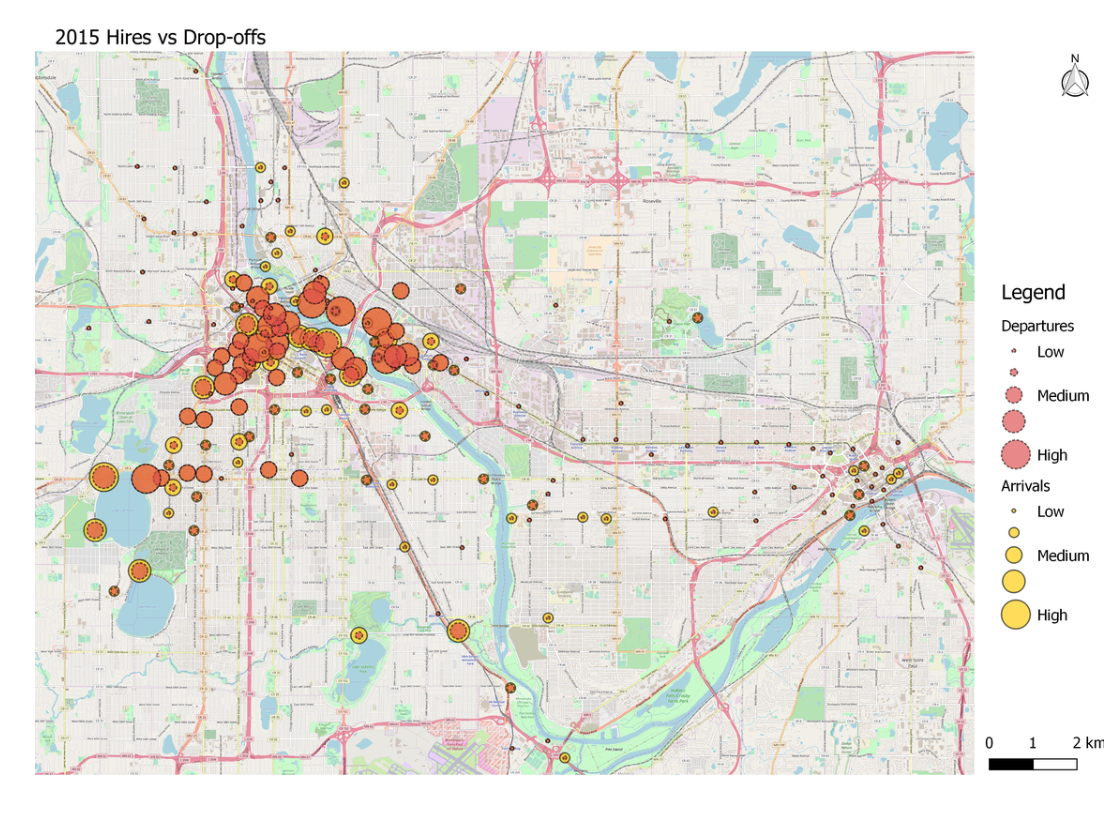
\includegraphics[scale=0.36]{figs/first_viz.PNG}
	\caption{\footnotesize{Mapping hires and drop-offs by circle area. \cite{UrbanDataCyclist}}}
	\label{fig:First viz Chart}
	\captionsetup{justification=centering,margin=1cm}
	\vspace{-10pt}
\end{figure}
\newline
This choice of visualization adheres with much of the design principles studied in our class. It follows the principle of effectiveness as the data is easily separable. By using a single channel (color) to distinguish between hires and drop-offs of bikes is more effective than using 2 channels for it. Also, we were planning to make this an unconstrained navigation which allows more freedom to the user to navigate. On the topic of task abstraction, this visualization is suitable to locate areas of high business activity. The area of circle directly correlates with the idea of high business volume.

In addition to that, the choice of color itself (red and blue) are easy to distinguish and hence are easily separable. These colors do not generally mesh with the mostly green and gray geographical background as well. This choice of visualization helps in the comparison between the hire data and drop-off data. In addition to that, it also helps in comparing the same kind of data (hires or drop-offs) with each other based on different locations. One drawback of this visualization is that the area of the circle does not give a quantitative value of the frequency of hires/drop-offs from the visualization itself. 

\subsection{PassType Mapping with Time}
\label{sec:viz2}

One of the things we were interested in the bike-sharing data was analyzing the bike pass types and their trend. For the bike-sharing service we chose, there are 3 kinds of passes -- daily, monthly and annual. Analysis of these bike-passes with a time of different granularity was not found in other visualization projects and research papers. This encouraged us to take on this concept to find some pattern or trend with this data. 

For this visualization, we planned on using line graph how the number of passes of each kind being bought for different levels of time granularity. The granularity levels could be a month, quarter or year. This option could be selected by the user from a drop-down box to the right of the line graph. Within the line graph, three lines represented the three types of passes. The choice of colors was red, blue and green. This triplet of colors form the basis of the RGB-colorspace which goes to prove that they are distinct from one another when used together. 

The X-axis would be the time axis and the Y-axis would be the magnitude axis. Here, the task abstraction shifts more towards the discovering and analyzing side. Our aim was to find some sort of trend moving forward with time. We expected to see an increase in monthly passes and a slight increase in annual passes. This would indicate that the bike-sharing service is getting popular with time. A more visible change could be perceived if the time was on a level of the year. On the other hand, the daily passes data would give a whole different perspective on how people use these services. By generalizing weather over months i.e. December-March for Winter, we could check if fewer people use the service during winters and more during spring/summer. 

In addition to the task abstraction, this visualization followed the principles of effectiveness and expressiveness as well. It is clearly distinguishable and it encodes only the required values. Being line graph, the level of accuracy is pretty good. Here, we have applied the principle of superimposing by overlaying the line graph of all 3 pass types into a single chart. Our assumption was that this number of overlay won't harm the distinguishability of the lines. Allowing the user to change the time granularity also helps in bringing user interactiveness into the picture. A rough sketch of what the visualization would probably look like is given below:
\begin{figure}[h]
	\centering % avoid the use of \begin{center}...\end{center} and use \centering instead (more compact)
	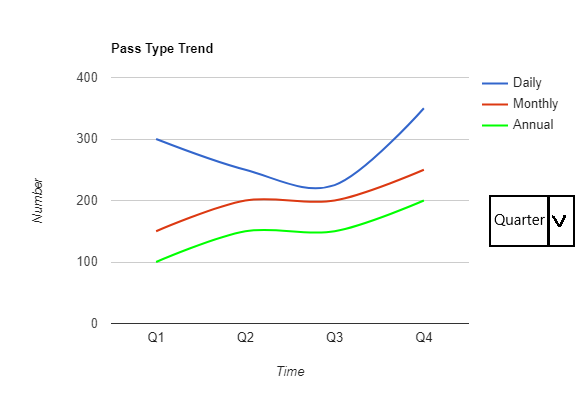
\includegraphics[scale=0.45]{figs/bar-graph.png}
	\caption{\footnotesize{Mapping of pass type with time granularity}}
	\label{fig:Second viz Chart}
	\captionsetup{justification=centering,margin=1cm}
	\vspace{-10pt}
\end{figure}
\newline

\subsection{Crossfilter Based Geographic Mapping}
\label{sec:viz3}

For the final design, we thought of implementing a crossfilter enabled geographic mapping of data. Basically, we will be expanding on the first visualization choice in this list. The difference here is that in the first visualization, the time range has been fixed beforehand. So there is no user interactivity in that visualization. On the other hand, this visualization adds a dynamic element to the previous static visualization. Here, we will have a geographic map just as in the first choice. We plan on mapping the drop-offs and hires just like in the first visualization. The data represented in the geographic plane can be controlled by a slider that can move through a time histogram. The time histogram will map the average duration of a trip for that period of time. So in this way, we can get even more insight into the trend in bike-sharing services.

By averaging the trip duration over a month, and creating a histogram with time as the X-axis and time in minutes as the Y-axis we can look for trends in the trip duration with respect to time. This can give us insights over the fact if people tend to use the bike-share for a longer duration during the summer over the winter. The trip duration might end up being completely independent to the month of the year as well, which is another observation in its own. 

Here, the geographic data can be used to check whether the station placement is optimum or not. If there are more high-frequency drop-offs and hires in a specific location, increasing the bike count in those areas might increase service even more. The histogram is in itself a good visualization and follows the basic design principles pretty well along with providing a high level of accuracy to data and a good form of comparison between data. Furthermore, filtering the geographic data with time gives us an idea of how frequently the bike-sharing service gets used with respect to time. This helps us in our task abstraction defined in the previous section. In addition to all this, having the means to interact and change data in real time is highly user-friendly and will be user-accepted as well. Below is a general mock-up of how the visualization might look like.
\begin{figure}[h]
	\centering % avoid the use of \begin{center}...\end{center} and use \centering instead (more compact)
	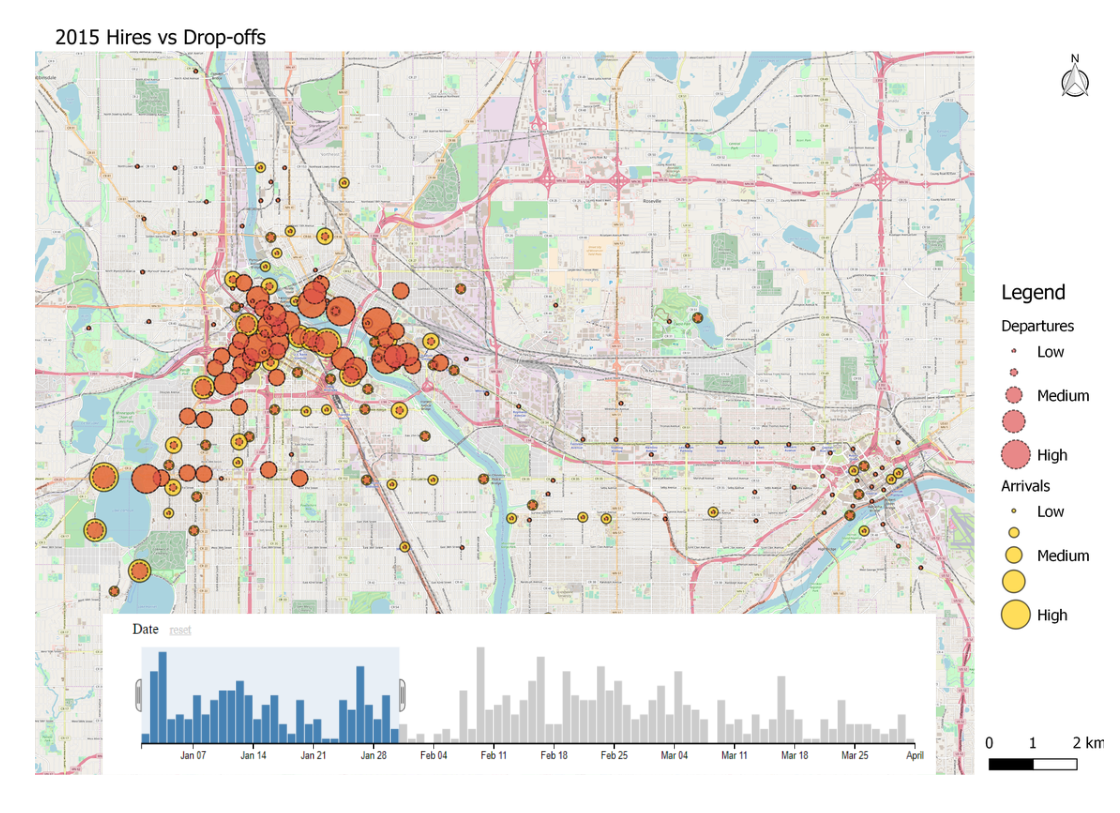
\includegraphics[scale=0.35]{figs/third_viz.PNG}
	\caption{\footnotesize{Crossfilter Enabled Mapping}}
	\label{fig:Third viz Chart}
	\captionsetup{justification=centering,margin=1cm}
	\vspace{-10pt}
\end{figure}

\subsection{Chosen Design}
\label{sec:viz4}

After considering all three visualizations based on their effectiveness, ease-of-use, complexity, and user-friendly interface, we decided to choose the third visualization \textbf{Crossfilter Enabled Geographic Mapping} as our chosen design. This visualization incorporated a number of different task abstractions viz. \textbf{comparison} between stations, \textbf{discover} trip duration in the histogram and maybe even \textbf{identify} outlier stations. This kind of visualization can be thought of as a focus + context design. When a certain area of time is highlighted, the remaining histogram greys out to denote that it is not included in the filter. Such design choices increase the effectiveness of the visualization. We also believe that using the real-time filter will adhere more to test volunteers who will find the visualization more interactive. Since users testing is a major part of our evaluation process, this result should definitely be taken in a positive vein.

%%\section{Technical Progress} 
\label{sec:technical_progress}

Continuing from the progress in the second milestone, we started implementation of the chosen visualization design. This involved a number of steps that were carried out over the course of two weeks that resulted in a visualization that now forms the basis of our future progress. The contributions made in service of this visualization design are explained in separate subsections below,

\subsection{Data Collection}
\label{sec:data collection}

The data used for the visualization was collected from the database of \textbf{Bike Share Metro}, a bike share service based in Los Angeles. This is a completely open source data that provides us with various information about any single bike ride. A more detailed description of all the fields in the data can be found in the Task Abstraction subsection of the Refinements section.\\
The data is divided into several segment, each one contained the information for a single quarter of a calendar year i.e. Q1, Q2, Q3 or Q4. After downloading the data from their online database, the resulting .zip archive was extracted. The raw data was provided in a CSV (Comma Separated Value) format.

\subsection{Data Refinement and Restructuring}
\label{sec:data refinement and restructuring}

The raw data in the CSV format is not suitable for processing and analysis. We used a more standard approach to work with data and for this the CSV data files were converted into JSON (JavaScript Object Notation) format. All of the data cleaning and pre-processing was done using the \textbf{Python} programming language. This reformatting of the raw data structure was followed by a series of further transformation which are explained in the sub-sections below.

\subsubsection{JSON Format}
As mentioned above, the first step was to convert the raw data from CSV to JSON format. Other than the structure of the data, the contents were left intact and no further manipulations were done to the data.\\
The script \texttt{csv\_to\_json.py} in the \textbf{Project} folder performs this initial conversion.

\subsubsection{GeoJSON Format}
While the JSON data format in itself is pretty suitable for data analysis and works very well for our purposes, GeoJSON is a format that works even better when visualizations involve geographic maps and latitude, longitude locations. During this process, we also performed data cleaning operations where data containing incomplete information were not loaded into the GeoJSON data structure.\\
The script \texttt{json\_to\_geojson.py} in the \textbf{Project} folder converts the JSON file into a GeoJSON data structure.

\subsubsection{Task-Specific Formats}
Following the GeoJSON re-formatting and data cleanup, the data structures for specific visualization mappings are created. The GeoJSON file is taken as the base file from which all other dictionaries and arrays of information are extracted.\\
For our current visualization progress, we have a single extraction from the GeoJSON file. This dictionary contains the distinct geographic locations of all bike pickup points along with the number of pickups for that time frame (1st quarter of 2018 in our case). This is done by the \texttt{geo\_to\_startcount.py} script in the \textbf{Project} directory.\newline\\ It should be noted that for every new visualization design or task, a new data structure will be extracted from the GeoJSON file to ease the data analysis and extraction process.
Currently, all these scripts exists in standalone and need to be executed one after the other. On the final implementation, these scripts will be a part of a single executable script which will perform all the data cleaning and manipulation tasks in a single execution.

\subsection{Data Visualization}
Following the data collection and restructuring, we proceeded towards the actual visualization of the data. The visualization process along with the different tools and packages used in support of that have been explained in the subsections below.

\subsubsection{Initial Map Layout}
The first task at hand was to lay out a map of Los Angeles over which we had to plot our data points. Though D3 in itself supports drawing maps, we required a detailed street level map layout. For this purpose, D3 could not be used alone. We had to use a separate package or library that supports interactive map drawing. We had two possible options to work with for our visualization, \textbf{Google Maps API} and \textbf{Leaflet}.\\
There did not seem to be a large difference between the functionalities provided by Google Maps and Leaflet, at least for our visualization purposes. While Google Maps did was a fan favorite among a large number of developers and it did provide many added features in terms of traffic, transit data and geolocation, we decided to implement Leaflet into our project. Our decision was based on the availability and simplicity of the documentation and tutorials for these features. Leaflet conformed to our requirements smoothly and its implementation was pretty straight forward.\\
In essence, Leaflet is a open-source JavaScript library for interactive maps \cite{Leaflet:2017:Doc}. It is light weight and consists of a plethora of features that can be implemented for interactive map visualizations. For our visualization, we create the map in the 'map' div and add \textit{OpenStreetMap} tiles to load the map area. As a starting point, we provide the map with a fixed co-ordinate and a zoom level. Using this information, an initial visual representation of the map is obtained. From here, users can further interact with the map. The interactions supported in our visualization are discussed in detail in a later section.
\begin{figure}[h]
	\centering % avoid the use of \begin{center}...\end{center} and use \centering instead (more compact)
	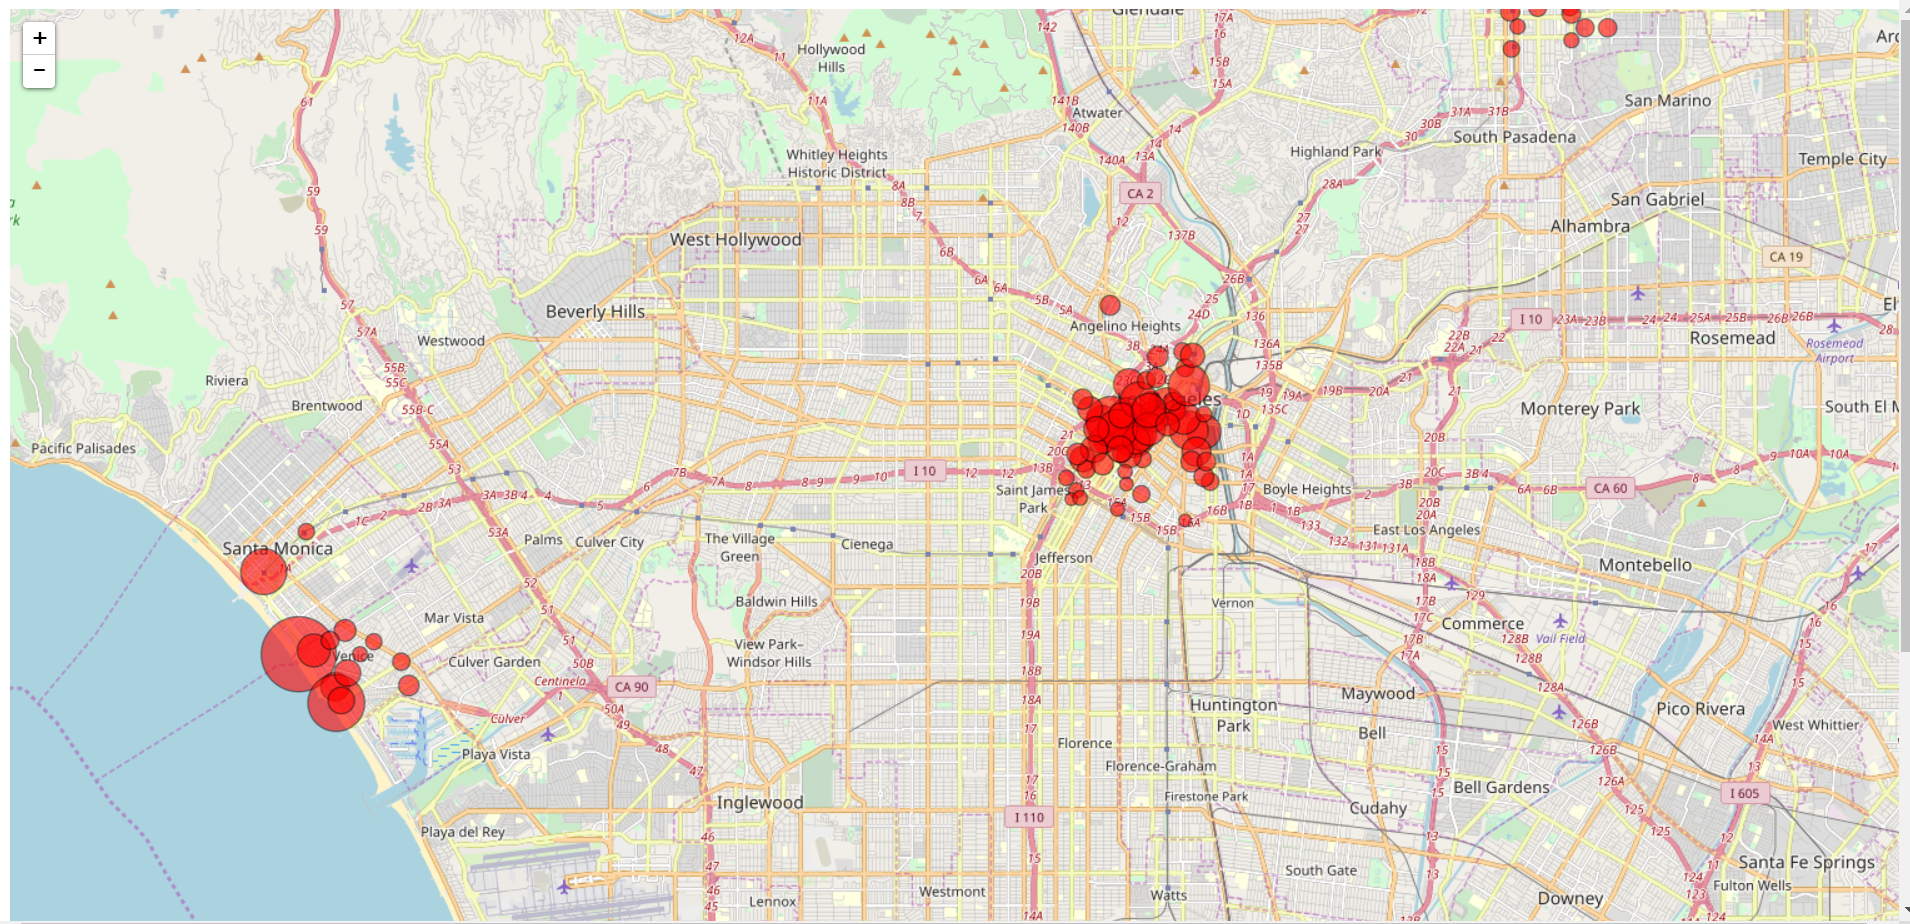
\includegraphics[scale=0.20]{figs/highlevel.PNG}
	\caption{\footnotesize{A high-level overview of current visualization}}
	\label{fig:First viz Chart}
	\captionsetup{justification=centering,margin=1cm}
	\vspace{-10pt}
\end{figure}
\subsubsection{Data Plotting}
After plotting the map of Los Angeles, we started with plotting the data points over this map. For the first visualization, we plotted the starting locations of all bike rides over the map. These were distinct locations in the map, defined by a latitude and longitude value. We used the data for the 1st quarter of 2018 as our seed data. The number of data points were in the order of 60,000 for a single quarter. For now, this data is loaded locally but as we include more data points for different quarters and years, we are planning to shift the data loading through a web server. This will considerably decrease the load time of the visualization.\\
The data points for our visualization are represented as circles of varying area (radius). The data is encoded in such a way that the radius linearly increases with the frequency of bike pick-ups for a given location. We keep the opacity of the circles to a value less than 1 so as to make the map visualization easier to understand and navigate. These circles are stroked with a minimum thickness to make them stand out when viewing from a zoomed-out perspective.
\begin{figure}[h]
	\centering % avoid the use of \begin{center}...\end{center} and use \centering instead (more compact)
	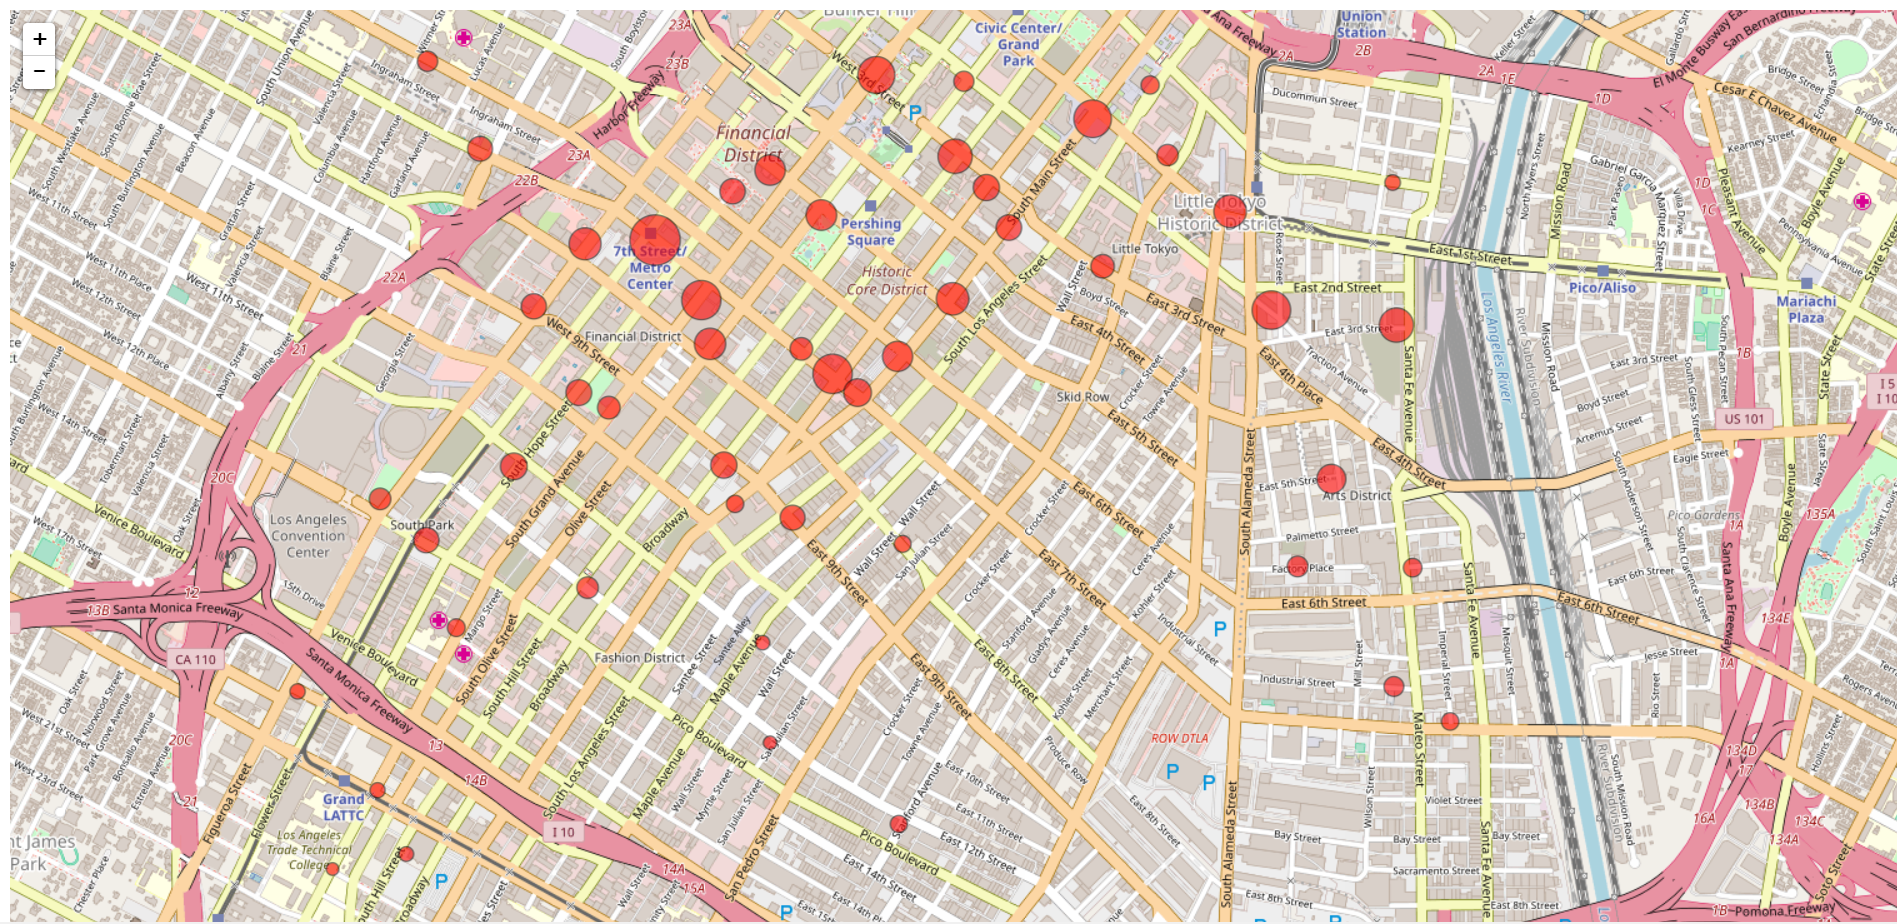
\includegraphics[scale=0.20]{figs/zoomedin.PNG}
	\caption{\footnotesize{A zoomed in view showing distinct geographic points}}
	\label{fig:First viz Chart}
	\captionsetup{justification=centering,margin=1cm}
	\vspace{-10pt}
\end{figure}
\subsection{User Interaction}
Our visualization design currently supports a number of interactions. These visualizations have been presented in the short movie as well. As work progresses on the visualization, these interactions will be enhanced and others added. For now, the following interactions are available to the user:
\begin{itemize}
    \item \textbf{Panning and Zooming}: The geographic map can be panned sideways to move around and locate different data points around the city. Also, the map can be zoomed in and out. Zooming in allows users to get a closer look into the data points on a street level view. This way the bike stations look more distinguishable from one another. The zoom feature here is constrained and semantic in nature. This interaction follows the Shneiderman's mantra of having an overview first and then allowing to zoom in and filter data.
    \item \textbf{Pop-up Effect}: The individual data points support a "On Click" feature. Every time a data point i.e. a circle is clicked, the color of the circle changes to blue with a more defined stroke around the circle. This makes the data point more visible and allows it to stand out, especially when there are a large number of similar data points around it. We decided on choosing the "On Click" action to show the effect rather than the "Hover" action since clicking an element to have a detailed overview of a single data point is more effective than hovering over it. Either ways, this follows the Shneiderman's Detail-on-Demand task taxonomy.
    \item \textbf{Tooltip}: In addition to the "On Click" feature changing the color of the circle, a tooltip will also appear on top of each data point. Currently, this tooltip shows the number of bike pick ups for a given location but a future enhancement might be to add a small visualization pertaining to the data within that geographic point.
\end{itemize}
\begin{figure}[h]
	\centering % avoid the use of \begin{center}...\end{center} and use \centering instead (more compact)
	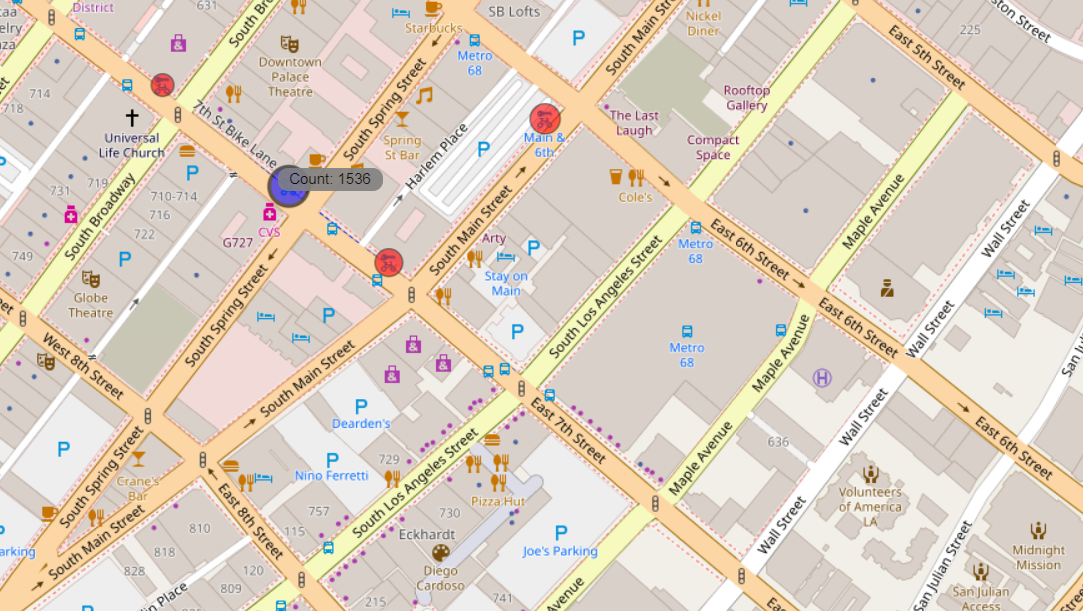
\includegraphics[scale=0.36]{figs/tooltip.png}
	\caption{\footnotesize{A simple tooltip implementation}}
	\label{fig:First viz Chart}
	\captionsetup{justification=centering,margin=1cm}
	\vspace{-10pt}
\end{figure}
This visualization has been coded by dividing the structure of the program into 3 segments:
\begin{itemize}
    \item PM3.html
    \item PM3.js
    \item PM3.css
\end{itemize}
As work progresses on the visualization, we plan on adding a histogram time frame at the bottom of the visualization window. This histogram will stretch the width of the window and allow users to cross-filter data in the map based on the selection in the histogram window.

\section{Refinements from Previous Milestone} 
\label{sec:research}

The second project milestone needed changes and improvements in the task abstraction section of the project. Much of these changes have been incorporated into this milestone. 

\subsection{Task Abstraction}
\label{sec:task abstraction}

We initially obtained our data from a popular online data source, Kaggle. The dataset was named \textit{Los Angeles Metro Bike Share Trip Data}. Even though this dataset had enough depth to reason about various trends and patterns, it was less in number which made us look for other sources of similar data. We then found a substantial amount of data in Bike Share Metro's database. Bike Share Metro is a bike sharing service providing in services in Download LA, Port of LA and Venice. This data seemed to fulfill our requirements for this project. This data, like the one before, is from \textit{Los Angeles} and contains the shared bike ride information for nearly 2.5 years, 2016 Q3 to 2018 Q3. 

The structure of the data sources provides the details of where and when journeys are made. In the below mentioned data-sets we have four spatial attributes namely, start\_lon, start\_lat, end\_lon and end\_lat. The data-set has a total of 14 attributes and they are as follows: 
\begin{itemize}
    \item trip\_id - Unique ID for a particular trip - This is of type integer
    \item duration - Duration of the trip in minutes - This is of type integer
    \item start\_time - Start time of the trip - This is a timestamp in format mm/dd/yyyy hh:mm
    \item end\_time - End time of the trip - This is a timestamp in format mm/dd/yyyy hh:mm
    \item start\_lon - Starting position longitude - This is of type float
    \item start\_lat - Starting position latitude - This is of type float
    \item start\_station - The station ID where the trip originated - This is of type integer
    \item end\_station -  The station ID where the trip terminated - This is of type integer
    \item end\_lat - Destination latitude - This is of type float
    \item end\_lon - Destination longitude - This is of type float
    \item bike\_id - Id for each bike - This is of type integer
    \item plan\_duration - Duration of the customer's plan - This is of type integer
    \item passholder\_type - The name of the pass holder's plan like "One Day Pass" or "Monthly Pass" or "Walk-up" or "Flex Pass" - This is of type string
    \item trip\_route\_category\ -  "Round Trip" for trips starting and ending at the same station or "One Way" for all other trips - This is of type string
\end{itemize}

In order to create a new design process model for data visualization, we utilized our team’s combined experience in visualization design as well as the concepts from existing models as a guide to identify different stages and components of the process. As a redesign team, we identified the goals, and tasks employed in an iterative process for our own visualization project. 

In our first milestone we understood the needs of bike share systems and identified the related data from Metro Bike share on which we could work on to identify the tasks. In our second milestone we ideated several new designs by many discussions among ourselves to generate a plethora of concepts and then winnow these into good ideas to better visualize the bike share system. In our third milestone we have finalized upon a single visualization design which we have decided to work on. This design incorporates various visualizations within a single frame that are layered in an interactive manner. These prototypes must be built to handle and visualize real data-sets, and it is common that, as prototypes get constructed, more design requirements or ideas may be explored and discovered, highlighting the iterative nature of visualization design. Another aspect of the make activity goes beyond design i.e. to employ software engineering and development techniques for writing code and programs to build visualizations to meet the needs of the users. We are using JavaScript, D3.js to build and generate interactive visualizations from the ground up. In the final milestone we have the final design activity in the visualization framework i.e. the deploy activity, with the motivation to construct a visualization system and bring it into effective action in a real-world setting in order to support the goals. The overall visualization artifact of this activity is a usable visualization system. This activity is the ultimate goal of problem-driven visualization design since it supports real-world users in their own work environments. 

 We applied Shneiderman's task taxonomy\cite{Shneiderman:1996:Mantra} to further drill down on the tasks we need to do. As per this taxonomy we first get the overview of the data we have with us. Based on this our main focus is on the number of customers, duration of their trips and the locations from which the bikes are rented. We zoom in on the tasks which interest us to analyze which places see the maximum number of business each day, and to see how the business is growing over time. We filter out the uninteresting data which is not of use in constructing the visualization (like bike station IDs). We can get more details-on-demand by first, panning and zooming into specific geographic locations in the map and then, clicking or hovering over data items in the map which bring up tooltips to display information specific to a location or a single bike ride. In this process we can retrieve the data required for our analysis. By following the above taxonomy so far we could classify our goals into the following:

\begin{itemize}
    \item G1: Get a mental picture of business according to location:
    It will be very helpful in analyzing the viability of the bike share system if we could get a mental picture, around which geographic locations most of the business tend to gather. If there was a visible comparison between different locations, it would be so much easier to comprehend where the focus of the business should be, moreover if we can find some connection between high volume of the rentals at those locations, the same model could also be implemented in other locations with similar potential. The idea of business can be explained by the number of drop-offs and hires from a specific station. Typically, a station having a high number of hires has more business. We will also check for stations where both drop-offs and hires are high. These can be considered as locations with high business. By mapping the drop-off i.e. (end\_longitude, end\_latitude) and hire i.e. (start\_longitude, start\_latitude) over the geographic map, we can get a good sense of our task.

    \item G2:  How the customers’ preferences are changing over time
    There are three kinds of passes available for the customers, namely walk-up (daily), monthly and flex (annual). They provide one day, one month and year-round rental service respectively. If we could find the trends in the change in the number of passes over different time granularity, we could get a clear picture of the preferences of the customers. The time granularity can be either months or quarters or years.
    
    \item G3: How the volume of the rentals changes over time:
    If we can visualize how the number of customers changes over time, it will also provide us with clarifications about which time of the year people tend to chose this form of transport over others. That would be beneficial to understand what compels them to eschew bikes over the other time of the years and what steps could be taken to alleviate their discomfort.
 
\end{itemize}
\\
To identify the smaller task in support of the goals, we can take the following steps.

\begin{itemize}
    \item T1: Getting the overview of the data: 
    First we must identify all the stations from their longitude and latitude over the city of Los Angeles. This will give us an insight about how all the renting stations are spread over the city. And moreover, if there is a heavy density of stations in some particular locations, we can then analyze how well individual stations are performing in that heavy cluster and can come to decisions about whether some stations may be relocated in some other location where the density of the stations is relatively low.

    \item T2: Cross-filter Based Geographic Mapping:
    This visualization adds a dynamic element to the previous static visualization. We plan on mapping the drop-offs and hires just like in the first visualization. The data being represented in the geographic plane can be controlled by a slider that can move through a time histogram. This way we can get an analysis of the data from nearly 2.5 years which will give us clear insight of the growth/decline of the business model over time.

    \item T3: Comparing the details of customer preferences of the passes throughout the years:
    We can make the comparisons between the different kinds of passes over different quarters/months of different years. We can show this way how many passes from the three categories are getting sold each at each time level. Moreover, it can give us some insights about which pass generates the most amount of revenue and which one is the best option for holding on to customer loyalty and thus garnering and maintaining the reputation for the company.
\end{itemize}

\textit{Summary}: All the visualizations necessary here tend to focus on the comparisons, discovery, and identification to some extent. We can use these task abstractions and objectives as further guides to our design selection process.

\section{Schedule} 
\label{sec:schedule}

For the second project milestone, we started off by trying to complete the proposed goals that were listed in the first project milestone. Following are those proposed goals:
\begin{enumerate}
    \item Finalize on the dataset for visualization
    \item Perform data cleansing and abstractions, categorizing them in the order in which they are mapped
    \item Discuss and agree on detailed work division for the project
    \item Perform initial visualization sketches
    \item Decide on the feasibility of current visualization ideas and add/remove as required
\end{enumerate}

Out of the five proposed goals, all goals except the second goal were completed. We were able to finalize on a dataset to be used for the project. There are a lot of open-source bike-sharing datasets available to choose from and most of them have the same set of attributes. We decided to go with the BikeShare Metro Los Angeles dataset.
We also discussed and agreed upon a detailed work division for the project. This task cannot be checked off as completed finished right now because we are still flexible about our task division. But what we have done is, agreed upon each member being the go-to person for a specific topic or application no matter who might be working on it. This results in every member being a spokesperson for one(or more) sections but still working together as a team.
Initial visualization sketches about what our visualization might look like at the end of the project were also made. Finally, we discussed and decided on the feasibility of our current visualization ideas. Through this process, we added the visualization which we eventually selected as the primary visualization for our project. Also, we decided that mapping the weather data should be kept as a future optional milestone and be done only if we had time.

We were not able to perform cleansing of our data and also did not categorize them in the order in which they are mapped. The primary reason for our inability to complete this goal was our lack for foresight when we planned for the second milestone. Initially, we had assumed that we would be able to start with the data cleansing and management task for the second milestone but picking the final visualization took more time than expected for us. This was a challenge for us during the initial stages of research. We went through a lot of research materials and also consulted various visualization students regarding our ideas. After careful consideration, we came to an agreed conclusion.

In addition to this, deciding on the dataset and on the feasibility of our visualization from PM1 took more time than initially planned. Our plan to start writing code and working with data only after deciding on a final visualization was a bad choice since that in part led us to miss goal 2 in our milestone. We could have started working with data and performing initial cleaning and formatting to it since that is not dependent on our final choice of visualization. We will make sure to think about these scenarios and prevent them from happening in the remaining milestones.

\begin{table}[h]
%% Table captions on top in journal version
 \caption{Project Milestones}\vspace{1ex} % the \vspace adds some space after the top caption
 \label{tab:milestones}
 \scriptsize
 \centering % avoid the use of \begin{center}...\end{center} and use \centering instead (more compact)
   \begin{tabular}{p{2cm}|p{6cm}}
     Milestone & Description (\%)\\
   \hline
     PM3 & Perform initial data cleansing and formatting to make input reads more streamlined\\
         & Create basic geographic visualizations using maps of the desired location\\
         & First visualization mapping the busiest locations in the city complete\\
         & Initial work on panning and zooming started\\
     PM4 & Right panel of time frame histogram designed and working\\
         & Linking the left and right visualization complete\\
	     & Refined the interactions within a visualization\\
	     & Initial stages of evaluation started\\
	     & Started preparations for the class presentation\\
     PM5 & Evaluation process completed\\
         & Revised data analysis and visualization tuning because on evaluation feedback\\
         & Class presentation and report submission completed\\
   \end{tabular}
\end{table}


%\bibliographystyle{abbrv}
\bibliographystyle{abbrv-doi-hyperref}
%%use following if all content of bibtex file should be shown
\nocite{*}
\bibliography{PM3}
\end{document}

